

\section{On-sky target templates: ScopeSim\_templates%
  \label{on-sky-target-templates-scopesim-templates}%
}

Documentation: \url{https://scopesim-templates.readthedocs.io/}

Code Base: \url{https://github.com/astronomyk/ScopeSim_templates}

Continuous integration: \url{https://travis-ci.org/github/astronomyk/ScopeSim_Templates}

Author: Kieran Leschinski


\section{Functionality%
  \label{functionality}%
}

\texttt{ScopeSim\_templates} creates astronomical sources in a format (\texttt{Source} objects)
that can be used by the instrument simulator \texttt{ScopeSim}.

It is designed to be agnostic regarding the instrument/telescope details. At the moment
only the most representative astronomical sources are included, however more
can be added with relative ease.


\subsection{Source object interface%
  \label{source-object-interface}%
}

A \texttt{ScopeSim.Source} object is a 2+1D (x, y, lambda) description of an on-sky object.
As such, it needs to contain the following information:

\begin{itemize}
\item A spatial description of the flux distribution on the sky. Either in table form (point sources)
or in image/bitmap form (extended sources). The spatial description is internally stored as
an \texttt{astropy.table.Table} object (in case of point sources) or as a \texttt{astropy.io.fits.ImageHDU} object
(extended sources).

\item A spectral description with the absolute flux per unit of wavelength of the objects. The spectral
description is stored as a \texttt{synphot.SourceSpectrum} object.
\end{itemize}

We plan to add support for fits datacubes in the near future.

Composition of sources are possible, for example creating an stellar field around a galaxy.


\subsection{What is included in the package%
  \label{what-is-included-in-the-package}%
}

\texttt{ScopeSim\_Templates} contains several functions to generate \texttt{ScopeSim.Source} objects.
In general, the most basic and more used functions are currently included in the package.
We expect to collaborate with the community to increase the breath of possible astronomical
sources.

The \texttt{Source} functions are organized in subpackages for a better accessibility.
They include a

\begin{itemize}
\item A \texttt{.basic} subpackage that contains functions to generate stars, stellar compositions
(clusters, grids, etc) and basic galaxy descriptions

\item An \texttt{.advanced} subpackage that contains - mostly - community contributions. In this package
however, is possible to find advanced galaxy definitions, including a 3D velocity field.

\item A \texttt{.micado} subpackage which contains MICADO specific sources with the main purpose of pipeline
testing
\end{itemize}


\subsection{Installation%
  \label{installation}%
}

To install \texttt{ScopeSim\_templates} simply type:

\begin{quote}
\begin{alltt}
\begin{lstlisting}[frame=single]
pip install scopesim_templates
\end{lstlisting}
\end{alltt}
\end{quote}

For the development version please visit the github repository.

\texttt{ScopeSim\_templates} should run with \texttt{Python} versions 3.5 and above.


\subsection{Dependencies%
  \label{dependencies}%
}

The following dependencies are necessary to run ScopeSim\_templates``
installed.

\begin{itemize}
\item \texttt{numpy}

\item \texttt{scipy}

\item \texttt{astropy}

\item \texttt{synphot}

\item \texttt{PyYAML}

\item \texttt{pyckles}

\item \texttt{scopesim}

\item \texttt{spextra}

\item \texttt{synphot}
\end{itemize}


\subsection{Example%
  \label{example}%
}

\begin{enumerate}
\item A stellar cluster with a mass of 100 Msun, located at 1000pc and a core radius of 1pc. Currently only
age=0 is supported.
\end{enumerate}

\phantomsection\label{scopesim-templates-cluster}
\begin{DUclass}{code}
\begin{DUclass}{plot}
\begin{DUclass}{clear-figure}
\begin{quote}
\begin{alltt}
\begin{lstlisting}[frame=single]
import matplotlib.pyplot as plt
from scopesim_templates.basic.stars import cluster

# This creates the source
my_cluster = cluster(mass=100, distance=1000, core_radius=1)

# Plot the positions
table = my_cluster.fields[0]
plt.plot(table["x"], table["y"], ".")
\end{lstlisting}
\end{alltt}
\end{quote}
\end{DUclass}
\end{DUclass}
\end{DUclass}

\begin{figure}[H]
\noindent\makebox[\linewidth][c]{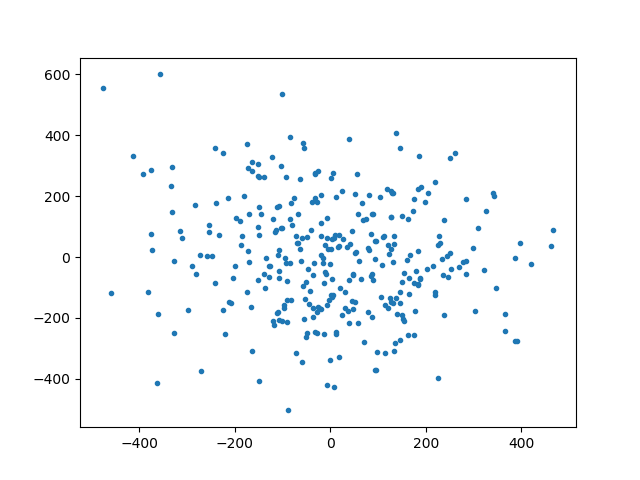
\includegraphics[scale=0.500000]{images/scopesim_templates_cluster.png}}\phantomsection\label{fig-scopesim-templates-cluster}

\caption{The positions of the cluster stars in arcseconds relative to the centre of the field of view .}
\end{figure}

\begin{enumerate}
\setcounter{enumi}{1}
\item A two component galaxy, with a younger component described by a star-forming spectra and an older by a
passive evolving spectral energy distribution
\end{enumerate}

\phantomsection\label{scopesim-templates-galaxy}
\begin{DUclass}{code}
\begin{DUclass}{plot}
\begin{DUclass}{clear-figure}
\begin{quote}
\begin{alltt}
\begin{lstlisting}[frame=single]
from scopesim_templates.basic.galaxy import spiral_two_component
import astropy.units as u

gal = spiral_two_component(fluxes=(20*u.ABmag, 21*u.ABmag))

plt.subplot(121)
plt.imshow(gal.fields[0].data)
plt.subplot(122)
plt.imshow(gal.fields[1].data)
\end{lstlisting}
\end{alltt}
\end{quote}
\end{DUclass}
\end{DUclass}
\end{DUclass}

\begin{figure}[H]
\noindent\makebox[\linewidth][c]{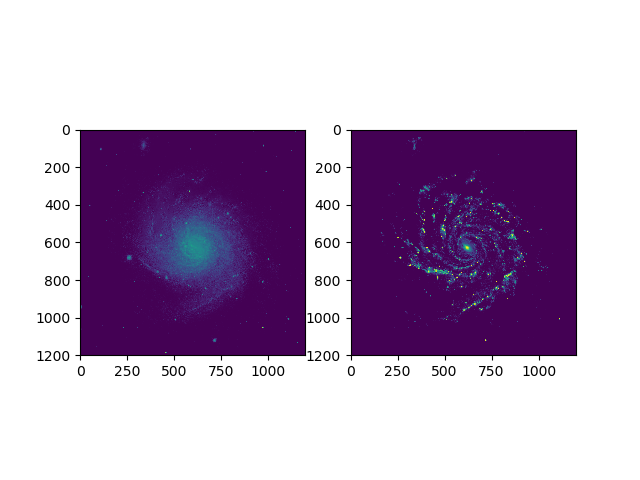
\includegraphics[scale=0.500000]{images/scopesim_templates_galaxy.png}}\phantomsection\label{fig-scopesim-templates-galaxy}

\caption{The two images which represent the new and old stellar populations of the spiral galaxy.}
\end{figure}

Above only the flux distribution on the sky can be appreciated. The description regarding the total flux
and its dependence with wavelength is contained in the \texttt{.spectra} property.

\phantomsection\label{scopesim-templates-galaxy-spectra}
\begin{DUclass}{code}
\begin{DUclass}{plot}
\begin{DUclass}{clear-figure}
\begin{quote}
\begin{alltt}
\begin{lstlisting}[frame=single]
gal = spiral_two_component(fluxes=(20*u.ABmag, 21*u.ABmag))
gal.spectra[0].plot(left=3000, right=8000, flux_unit="FLAM")
\end{lstlisting}
\end{alltt}
\end{quote}
\end{DUclass}
\end{DUclass}
\end{DUclass}

\begin{figure}[H]
\noindent\makebox[\linewidth][c]{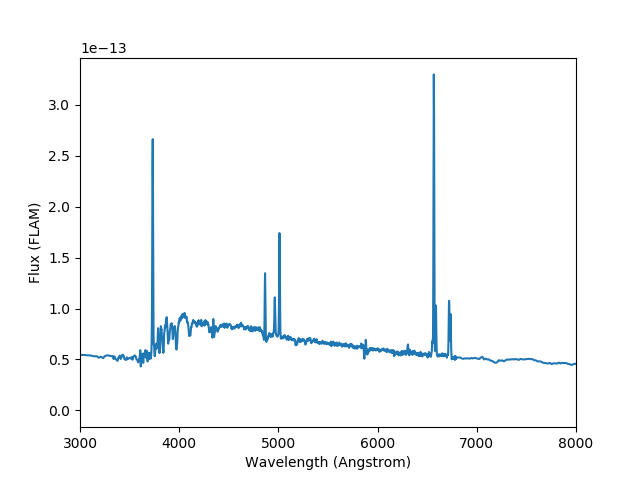
\includegraphics[scale=0.500000]{images/scopesim_templates_galaxy_spectra.png}}\phantomsection\label{fig-scopesim-templates-galaxy-spectra}

\caption{The spectra associated with each of the galaxy components}
\end{figure}


\subsection{Documentation%
  \label{documentation}%
}

\begin{itemize}
\item scopesim\_templates main documentation

\item source object interface documentation from scopesim-templates

\item converting from simcado to scopesim
\end{itemize}
